% --- [ System Architecture ] --------------------------------------------------

% <howto>
% * the overall structure of the software system (architecture)

% <howto>
% * Software architecture is concerned with deciding what has to be done, and which program component is going to do it (how something is done is left to the detailed design phase, below)
% * It effectively defines the interface between the programs of the system.
% * This stage does not need to consider non-functional requirements (e.g. response time, reliability, maintainability).

\subsection{System Architecture}
\label{sec:design_system_architecture}

The decompilation pipeline conceptually consists of three modules which separate the general decompilation tasks (e.g. control flow analysis) from concerns related to the source language and the target language. Firstly, the front-end translates a variety of source languages (e.g. x86 or ARM assembly, C or Haskell source code, …) to LLVM IR by utilizing several independent open source projects. Secondly, the middle-end structures the LLVM IR by identifying high-level control flow primitives in the CFGs generated from the intermediate representation. Lastly, the back-end translates the structured LLVM IR into a high-level target programming language (e.g. Go). The interaction between these modules is visualised in figure~\ref{fig:decompilation_pipeline}, and the individual components of the front-end, middle-end and back-end modules are further described in section~\ref{sec:design_front-end_components},~\ref{sec:design_middle-end_components} and~\ref{sec:design_back-end_components} respectively.

\begin{figure}[htbp]
	\begin{center}
		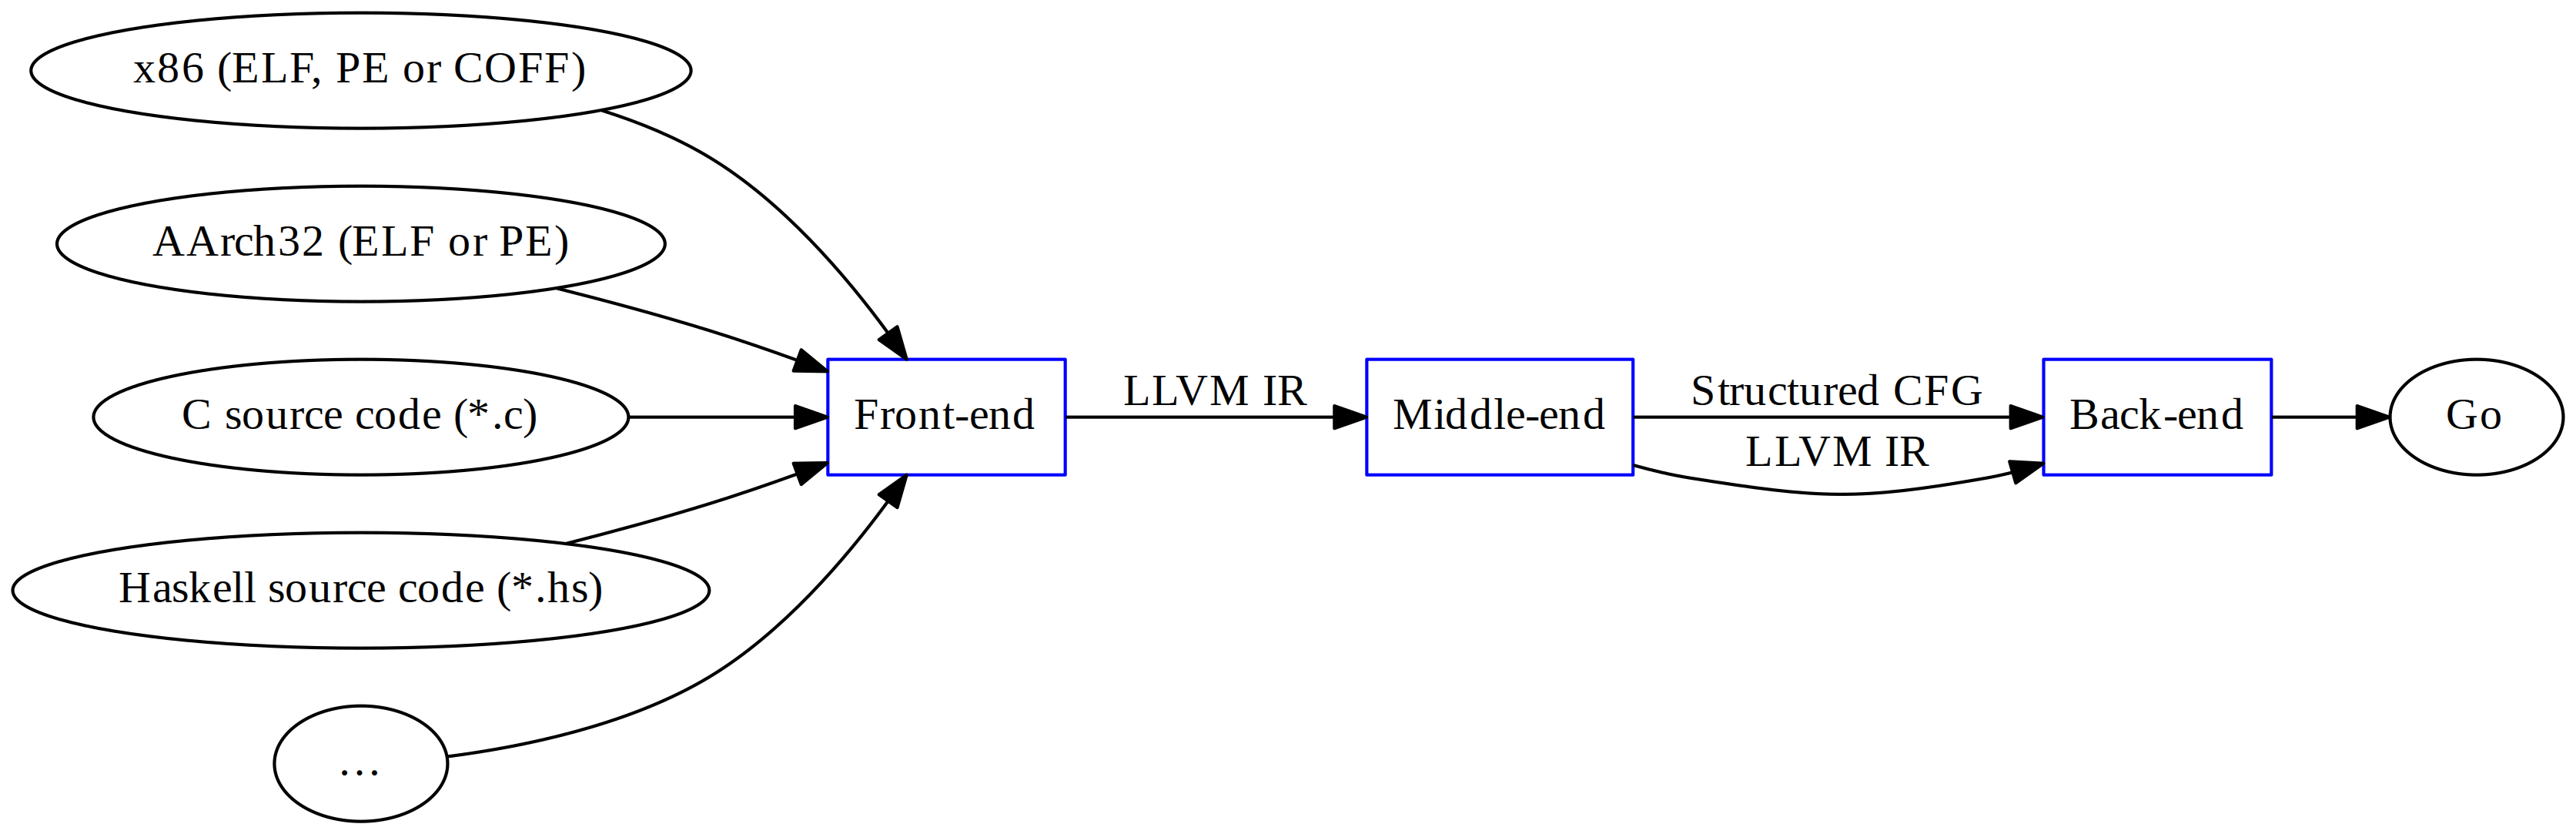
\includegraphics[width=\textwidth]{inc/6_design/decompilation_pipeline.png}
		\caption{The front-end of the decompilation pipeline translates a variety of inputs (e.g. native code or source code) to LLVM IR; the middle-end structures the LLVM IR through control flow analysis; and the back-end translates the structured LLVM IR to a high-level programming language (e.g. Go).}
		\label{fig:decompilation_pipeline}
	\end{center}
\end{figure}

The main benefit with this decompiler architecture is that it scales well when implementing support for additional source languages (e.g. MIPS or PowerPC assembly) and target languages (e.g. Python), as the general decompilation tasks only have to be implemented once. The decompiler architecture is an adaptation of the one presented by C. Cifuentes back in 1994 (as described in section~\ref{sec:lit_review_decompilation_phases}), which was heavily inspired by the architecture of compilers that separated general optimisation tasks (e.g. constant propagation) from concerns related to the source programming language (e.g. C) and the target computer architecture (e.g. x86). The compiler architecture has been proven so effective at separating concerns that it remains in use today by several production-quality compilers~\cite{llvm_architecture,gcc_architecture}.
